\subsection{Automatic Differentiation}
To demonstrate the automatic differentiation, 3 alternative methods were implemented to solve the following equation: 

\begin{equation}
    f(x) = \log(\sin(x)) + x^2 \cos(x)
    \label{eq:f}
\end{equation}

\subsubsection{Analytical Solution}
The analytical solution to Equation~\ref{eq:f} is: 

\begin{equation}
    f'(x) = \frac{\cos(x)}{\sin(x)} + 2x \cos(x) - x^2 \sin(x)
    \label{eq:f_prime}
\end{equation}

which equals -1.9123 at x = 1.5.

\subsubsection{Automatic Differentiation Solution}
To perform the automatic differentiation, the \texttt{Dual} class was used.
This yielded the a value of -1.9123 at x = 1.5, which is the same as the analytical solution.


\subsubsection{Numerical Solution}
To perform the numerical differentiation, the central difference method was used.
This was performed for a variety of step sizes, and the results are shown in Figure~\ref{fig:diff_demo}.
This method is defined as: 

\begin{equation}
    f'(x) = \frac{f(x+h) - f(x-h)}{2h}
    \label{eq:central_diff}
\end{equation}

The results compared to the other methods are shown in Figure~\ref{fig:diff_demo}.

\subsubsection{Timimg Comparison}
A benchmark was performed to compare the time taken (automatic and numerical differentiation), by performing the differentiation 1000 times, 
and averaging the time taken.

\begin{table}[h]
    \centering
    \begin{tabular}{|l|c|c|}
    \hline
    Method & Time (s) \\
    \hline
    Numerical & 0.003912 \\
    Automatic & 0.008927 \\
    \hline
    \end{tabular}
    \caption{Performance comparison of numerical and automatic differentiation}
    \end{table}

\begin{figure}[h]
    \centering
    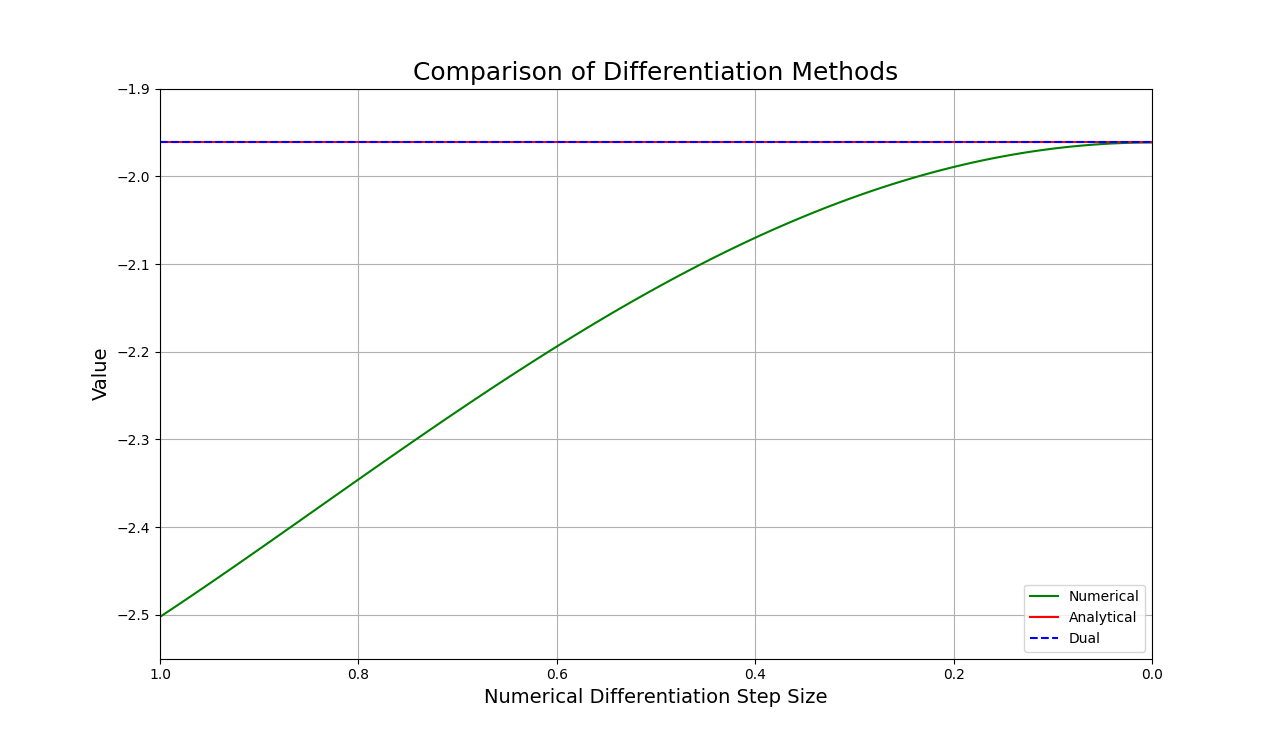
\includegraphics[width=1\textwidth]{images/diff_demo.png}
    \caption{Comparison of Differentiation Methods}
    \label{fig:diff_demo}
\end{figure}


\subsection{Cython Performance}
A benchmark study of the four basic operations was performed, with 1 million iterations between the Python and Cython versions.
Figure \ref{fig:basic_ops_speedup} shows the speedup of the basic operations, and Figure \ref{fig:basic_ops_memory} shows the memory use.

\begin{table}[h]
    \centering
    \begin{tabular}{|l|c|c|c|c|}
    \hline
    Method & Python Time (ms) & Cython Time (ms) & Python Memory (B) & Cython Memory (B) \\
    \hline
    Addition & 0.007000 & 0.012000 & 912 & 848\\
    Multiplication & 0.013900 & 0.014400 & 848 & 752\\
    Division & 0.024000 & 0.007200 & 880 & 720\\
    Derivative & 0.049900 & 0.007700 & 1120 & 784\\
    \hline
    \end{tabular}
    \caption{Time and Memory Comparison of Basic Operations}
    \end{table}

\begin{figure}[h]
    \centering
    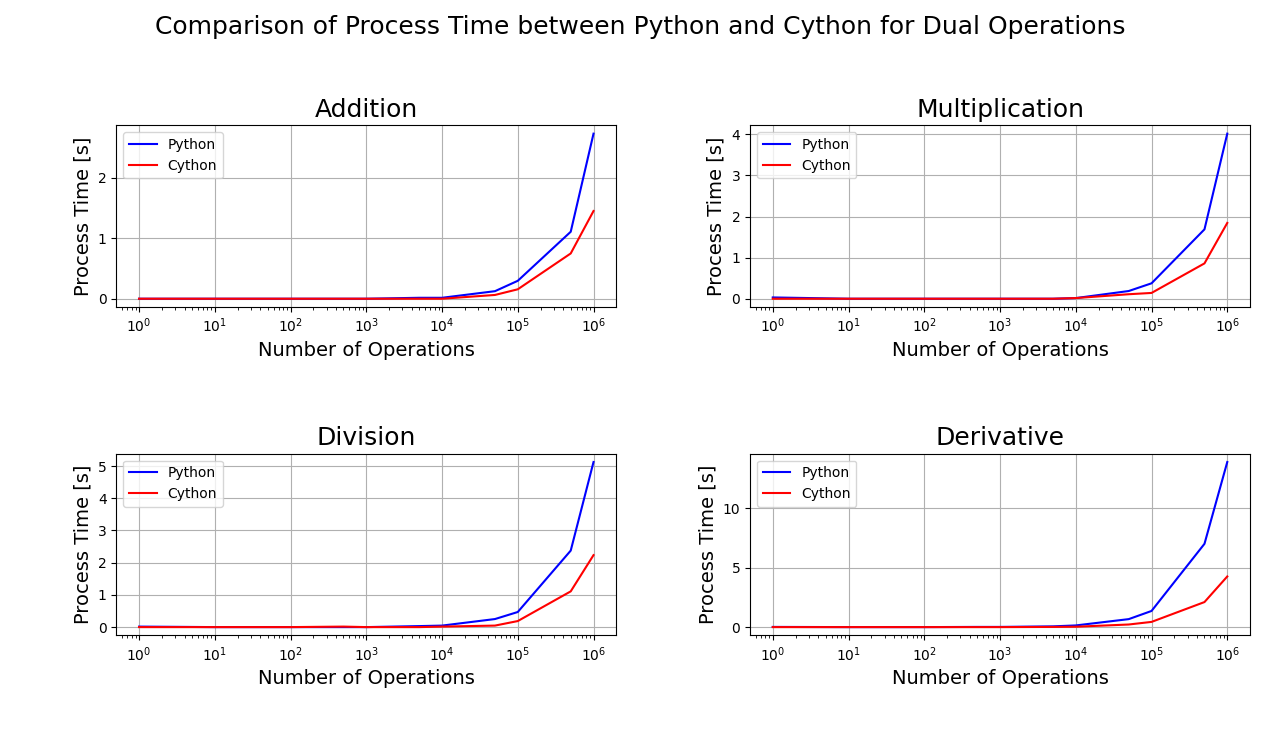
\includegraphics[width=1\textwidth]{images/basic_ops_speedup.png}
    \caption{Python vs. Cython Speedup for 1 million operations}
    \label{fig:basic_ops_speedup}
\end{figure}

\begin{figure}[h]
    \centering
    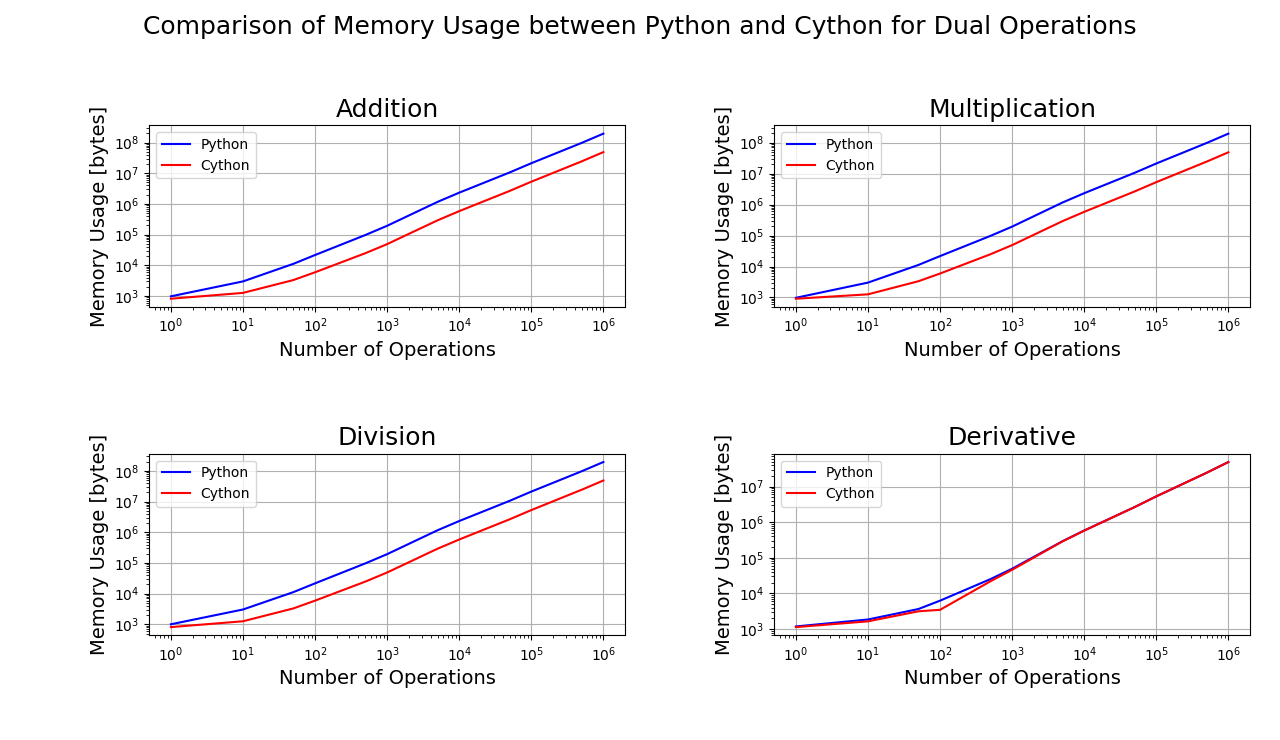
\includegraphics[width=1\textwidth]{images/basic_ops_memory.png}
    \caption{Python vs. Cython Memory Use for 1 million operations}
    \label{fig:basic_ops_memory}
\end{figure}

